\subsection{第 11 课 | 二分查找}

\subsubsection{脑图}

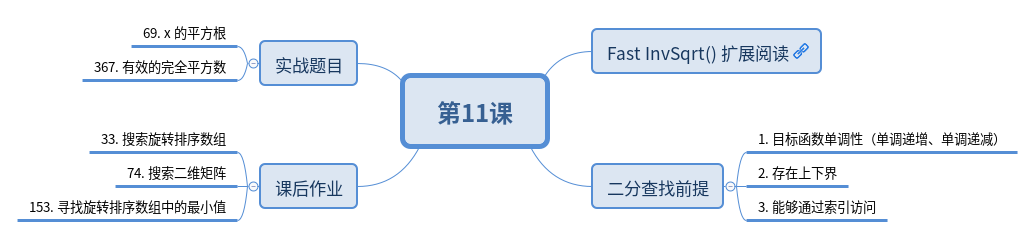
\includegraphics[width=170mm,height=80mm]{images/第11课.png}

\subsubsection{题目}

\paragraph{实战题目}

\begin{itemize}
  \item \hyperref[leetcode:69]{69. x 的平方根}
  \item \hyperref[leetcode:367]{367. 有效的完全平方数}
\end{itemize}

\paragraph{课后作业}

\begin{itemize}
  \item \hyperref[leetcode:33]{33. 搜索旋转排序数组}
  \item \hyperref[leetcode:74]{74. 搜索二维矩阵}
  \item \hyperref[leetcode:153]{153. 寻找旋转排序数组中的最小值}
  \item 使用二分查找,寻找一个半有序数组 [4, 5, 6, 7, 0, 1, 2] 中间无序的地方
    说明:同学们可以将自己的思路、代码写在第 3 周的学习总结中
\end{itemize}
